\section{Additional results}
\label{sec:s-results}

\subsection{Full metric panel (primary rule D1)}
Mean $\pm$ SD over five seeds (\%, except MCC and cost); TP/TN/FP/FN are the exact confusion-matrix counts of the seed-ensemble predictions on all \nSamplesEval{} outer-test samples. FPR $=1-$specificity and FNR $=1-$recall.

\noindent\resizebox{\textwidth}{!}{\begin{tabular}{lccccccccccccccc}
\toprule
Model & Acc. & Prec. & Rec. & Spec. & F1 & Bal.acc. & MCC & G-mean & FPR & FNR & Cost$_{5:1}$ & TP & TN & FP & FN \\
\midrule
E-DDQN & 45.4$\pm$1.3 & 44.4$\pm$0.7 & 93.4$\pm$2.5 & 7.4$\pm$2.7 & 60.2$\pm$0.9 & 50.4$\pm$1.2 & 0.016$\pm$0.054 & 26.0$\pm$4.5 & 92.6$\pm$2.7 & 6.6$\pm$2.5 & 0.663$\pm$0.048 & 3,747 & 423 & 4,820 & 400 \\
E-CB & 47.6$\pm$1.2 & 45.6$\pm$0.6 & 97.1$\pm$2.9 & 8.4$\pm$2.8 & 62.1$\pm$1.0 & 52.8$\pm$1.2 & 0.122$\pm$0.052 & 28.2$\pm$5.0 & 91.6$\pm$2.8 & 2.9$\pm$2.9 & 0.575$\pm$0.055 & 4,007 & 763 & 4,480 & 140 \\
DQN & 50.1$\pm$1.9 & 46.8$\pm$1.0 & 95.2$\pm$2.7 & 14.5$\pm$4.9 & 62.8$\pm$0.8 & 54.8$\pm$1.6 & 0.158$\pm$0.038 & 36.6$\pm$5.8 & 85.5$\pm$4.9 & 4.8$\pm$2.7 & 0.584$\pm$0.040 & 4,018 & 852 & 4,391 & 129 \\
CS-MLP & 45.4$\pm$0.9 & 44.7$\pm$0.4 & 99.4$\pm$0.7 & 2.8$\pm$1.9 & 61.7$\pm$0.4 & 51.1$\pm$0.8 & 0.072$\pm$0.049 & 14.7$\pm$8.8 & 97.2$\pm$1.9 & 0.6$\pm$0.7 & 0.557$\pm$0.012 & 4,124 & 318 & 4,925 & 23 \\
LogReg & 48.3$\pm$0.0 & 46.0$\pm$0.0 & 99.1$\pm$0.0 & 8.1$\pm$0.0 & 62.9$\pm$0.0 & 53.6$\pm$0.0 & 0.167$\pm$0.000 & 28.4$\pm$0.0 & 91.9$\pm$0.0 & 0.9$\pm$0.0 & 0.532$\pm$0.000 & 4,111 & 426 & 4,817 & 36 \\
HGB & 51.0$\pm$0.0 & 47.3$\pm$0.0 & 97.0$\pm$0.0 & 14.6$\pm$0.0 & 63.6$\pm$0.0 & 55.8$\pm$0.0 & 0.197$\pm$0.000 & 37.6$\pm$0.0 & 85.4$\pm$0.0 & 3.0$\pm$0.0 & 0.543$\pm$0.000 & 4,023 & 764 & 4,479 & 124 \\
RF & 53.6$\pm$0.3 & 48.8$\pm$0.2 & 98.5$\pm$0.3 & 18.2$\pm$0.7 & 65.2$\pm$0.1 & 58.3$\pm$0.3 & 0.266$\pm$0.004 & 42.3$\pm$0.8 & 81.8$\pm$0.7 & 1.5$\pm$0.3 & 0.491$\pm$0.003 & 4,093 & 962 & 4,281 & 54 \\
\bottomrule
\end{tabular}
}

\subsection{Secondary operating rules}
Mean $\pm$ SD over five seeds; FN and FP are the exact counts of the seed ensemble, as in the main text. In the two tables below, the name of the proposed model and the lowest cost among the primary models are set in bold. Rule D0 (untuned cut-off $\hat p\ge 1/6$, the nominal 5:1 Bayes cut-off; for the asymmetric agents the greedy policy; its effective position on $P(y=1\mid s)$ for each model is given in Section~S5.12):

\noindent\resizebox{\textwidth}{!}{\begin{tabular}{lccccccccccc}
\toprule
Model & Recall & Spec. & Prec. & F1 & Bal. acc. & MCC & Cost$_{5:1}$ & ROC-AUC & PR-AUC & FN & FP \\
\midrule
\textbf{E-DDQN} & 77.2$\pm$3.8 & 28.0$\pm$2.0 & 45.9$\pm$1.7 & 57.6$\pm$2.4 & 52.6$\pm$2.7 & 0.060$\pm$0.061 & 0.905$\pm$0.092 & 0.538$\pm$0.016 & 0.483$\pm$0.019 & 909 & 3,862 \\
E-CB & 85.9$\pm$2.2 & 37.2$\pm$3.0 & 52.0$\pm$1.1 & 64.7$\pm$1.1 & 61.5$\pm$1.5 & 0.258$\pm$0.031 & 0.663$\pm$0.044 & 0.653$\pm$0.011 & 0.562$\pm$0.006 & 627 & 3,262 \\
DQN & 85.1$\pm$1.7 & 37.1$\pm$1.5 & 51.7$\pm$0.7 & 64.3$\pm$0.9 & 61.1$\pm$1.0 & 0.248$\pm$0.022 & 0.680$\pm$0.035 & 0.661$\pm$0.013 & 0.595$\pm$0.022 & 561 & 3,330 \\
CS-MLP & 83.0$\pm$3.1 & 36.4$\pm$2.3 & 50.8$\pm$1.0 & 63.0$\pm$1.5 & 59.7$\pm$1.6 & 0.215$\pm$0.037 & 0.731$\pm$0.066 & 0.644$\pm$0.018 & 0.521$\pm$0.022 & 622 & 3,381 \\
LogReg & 85.3$\pm$0.0 & 13.6$\pm$0.0 & 43.8$\pm$0.0 & 57.9$\pm$0.0 & 49.4$\pm$0.0 & $-$0.016$\pm$0.000 & 0.808$\pm$0.000 & 0.626$\pm$0.000 & 0.576$\pm$0.000 & 611 & 4,531 \\
HGB & 92.0$\pm$0.0 & 30.0$\pm$0.0 & 51.0$\pm$0.0 & 65.6$\pm$0.0 & 61.0$\pm$0.0 & 0.272$\pm$0.000 & 0.567$\pm$0.000 & 0.692$\pm$0.000 & 0.593$\pm$0.000 & 331 & 3,670 \\
RF & 94.5$\pm$0.1 & 34.9$\pm$0.1 & 53.4$\pm$0.0 & 68.3$\pm$0.0 & 64.7$\pm$0.0 & 0.353$\pm$0.001 & \textbf{0.486$\pm$0.001} & 0.688$\pm$0.002 & 0.548$\pm$0.001 & 228 & 3,410 \\
\midrule
Always alarm & 100.0 & 0.0 & 44.2 & 61.3 & 50.0 & 0.000 & 0.558 & -- & -- & 0 & 5,243 \\
Never alarm & 0.0 & 100.0 & -- & -- & 50.0 & 0.000 & 2.208 & -- & -- & 4,147 & 0 \\
\bottomrule
\end{tabular}
}

\medskip
Validation recall constraint ($\ge$0.95 on pooled inner-OOF predictions):

\noindent\resizebox{\textwidth}{!}{\begin{tabular}{lccccccccccc}
\toprule
Model & Recall & Spec. & Prec. & F1 & Bal. acc. & MCC & Cost$_{5:1}$ & ROC-AUC & PR-AUC & FN & FP \\
\midrule
\textbf{E-DDQN} & 86.8$\pm$3.1 & 11.5$\pm$3.4 & 43.7$\pm$0.9 & 58.1$\pm$1.3 & 49.1$\pm$1.7 & $-$0.027$\pm$0.053 & 0.785$\pm$0.062 & 0.538$\pm$0.016 & 0.483$\pm$0.019 & 641 & 4,539 \\
E-CB & 95.2$\pm$2.7 & 15.0$\pm$3.3 & 47.0$\pm$0.8 & 62.9$\pm$1.0 & 55.1$\pm$1.4 & 0.167$\pm$0.042 & 0.581$\pm$0.051 & 0.653$\pm$0.011 & 0.562$\pm$0.006 & 317 & 4,093 \\
DQN & 93.5$\pm$2.9 & 23.0$\pm$3.4 & 49.0$\pm$0.8 & 64.3$\pm$1.0 & 58.3$\pm$1.2 & 0.227$\pm$0.032 & 0.573$\pm$0.052 & 0.661$\pm$0.013 & 0.595$\pm$0.022 & 343 & 3,810 \\
CS-MLP & 98.3$\pm$1.2 & 9.3$\pm$4.2 & 46.2$\pm$1.0 & 62.8$\pm$0.9 & 53.8$\pm$1.9 & 0.156$\pm$0.052 & 0.544$\pm$0.025 & 0.644$\pm$0.018 & 0.521$\pm$0.022 & 105 & 4,463 \\
LogReg & 97.2$\pm$0.0 & 18.3$\pm$0.0 & 48.5$\pm$0.0 & 64.7$\pm$0.0 & 57.7$\pm$0.0 & 0.241$\pm$0.000 & 0.518$\pm$0.000 & 0.626$\pm$0.000 & 0.576$\pm$0.000 & 116 & 4,285 \\
HGB & 97.5$\pm$0.0 & 18.3$\pm$0.0 & 48.6$\pm$0.0 & 64.8$\pm$0.0 & 57.9$\pm$0.0 & 0.248$\pm$0.000 & 0.511$\pm$0.000 & 0.692$\pm$0.000 & 0.593$\pm$0.000 & 103 & 4,282 \\
RF & 97.0$\pm$0.2 & 25.4$\pm$0.3 & 50.7$\pm$0.0 & 66.6$\pm$0.0 & 61.2$\pm$0.0 & 0.307$\pm$0.002 & \textbf{0.483$\pm$0.004} & 0.688$\pm$0.002 & 0.548$\pm$0.001 & 128 & 3,896 \\
\midrule
Always alarm & 100.0 & 0.0 & 44.2 & 61.3 & 50.0 & 0.000 & 0.558 & -- & -- & 0 & 5,243 \\
Never alarm & 0.0 & 100.0 & -- & -- & 50.0 & 0.000 & 2.208 & -- & -- & 4,147 & 0 \\
\bottomrule
\end{tabular}
}

\subsection{Group-bootstrap confidence intervals}
Seed-ensemble predictions, rule D1; 95\,\% percentile intervals from 2,000 bootstrap replicates of the \nGroupsEval{} linkage groups.

\noindent\resizebox{\textwidth}{!}{\begin{tabular}{lccccc}
\toprule
Model (seed ensemble, D1) & Recall & Spec. & Cost$_{5:1}$ & ROC-AUC & PR-AUC \\
\midrule
E-DDQN & 90.4 [77.7, 98.9] & 8.1 [1.5, 17.6] & 0.726 [0.533, 0.996] & 0.541 [0.382, 0.690] & 0.496 [0.329, 0.683] \\
E-CB & 96.6 [92.2, 99.6] & 14.6 [8.3, 21.4] & 0.552 [0.431, 0.673] & 0.659 [0.550, 0.767] & 0.565 [0.429, 0.740] \\
DQN & 96.9 [92.6, 99.7] & 16.3 [8.7, 24.8] & 0.536 [0.417, 0.654] & 0.665 [0.558, 0.785] & 0.606 [0.456, 0.778] \\
CS-MLP & 99.4 [98.5, 100.0] & 6.1 [2.6, 10.8] & 0.537 [0.421, 0.634] & 0.654 [0.527, 0.781] & 0.529 [0.393, 0.712] \\
LogReg & 99.1 [98.0, 100.0] & 8.1 [4.0, 13.0] & 0.532 [0.429, 0.627] & 0.626 [0.498, 0.750] & 0.576 [0.408, 0.754] \\
HGB & 97.0 [92.4, 99.9] & 14.6 [7.0, 24.9] & 0.543 [0.439, 0.654] & 0.692 [0.574, 0.809] & 0.593 [0.437, 0.779] \\
RF & 98.7 [97.5, 99.6] & 18.3 [11.7, 28.0] & 0.485 [0.381, 0.577] & 0.688 [0.582, 0.808] & 0.548 [0.443, 0.735] \\
\bottomrule
\end{tabular}
}

\subsection{Per-fold results}
Expected 5:1 cost / ROC-AUC of the seed ensemble in each outer fold (rule D1). Fold-to-fold variation is large because each fold contains only 3--5 linkage groups.

\noindent\resizebox{\textwidth}{!}{\begin{tabular}{lccccc}
\toprule
Model & Fold 0 & Fold 1 & Fold 2 & Fold 3 & Fold 4 \\
\midrule
E-DDQN & 0.604 / 0.536 & 0.762 / 0.522 & 0.529 / 0.734 & 1.184 / 0.501 & 0.693 / 0.466 \\
E-CB & 0.569 / 0.655 & 0.537 / 0.718 & 0.462 / 0.756 & 0.460 / 0.747 & 0.758 / 0.447 \\
DQN & 0.564 / 0.715 & 0.757 / 0.521 & 0.451 / 0.852 & 0.426 / 0.740 & 0.520 / 0.499 \\
CS-MLP & 0.604 / 0.575 & 0.542 / 0.596 & 0.495 / 0.820 & 0.528 / 0.708 & 0.501 / 0.659 \\
LogReg & 0.582 / 0.623 & 0.542 / 0.428 & 0.486 / 0.810 & 0.531 / 0.712 & 0.515 / 0.610 \\
HGB & 0.619 / 0.631 & 0.547 / 0.740 & 0.510 / 0.791 & 0.522 / 0.761 & 0.495 / 0.585 \\
RF & 0.600 / 0.630 & 0.463 / 0.728 & 0.397 / 0.771 & 0.457 / 0.761 & 0.486 / 0.685 \\
\bottomrule
\end{tabular}
}

\subsection{Event-level behavior}
Seed ensembles at rule D1. Alarm percentages are the fraction of seconds with an alarm in each session, averaged over sessions (before onset: the \nEventSessions{} sessions with an event; event-free: the \nEventFreeSessions{} sessions without one).

\noindent\resizebox{\textwidth}{!}{\begin{tabular}{lcccc}
\toprule
Model & Events detected & Median delay (s) & Alarm \% before onset & Alarm \% in event-free sessions \\
\midrule
E-DDQN & 26/26 & 0 & 82.3 & 96.6 \\
E-CB & 25/26 & 0 & 73.1 & 76.9 \\
DQN & 25/26 & 0 & 77.4 & 70.4 \\
CS-MLP & 26/26 & 0 & 92.9 & 88.1 \\
LogReg & 25/26 & 0 & 76.0 & 91.7 \\
HGB & 25/26 & 0 & 69.3 & 90.8 \\
RF & 25/26 & 0 & 61.3 & 75.3 \\
\bottomrule
\end{tabular}
}

\subsection{Paired tests under the secondary rules}
Rule D0:

\noindent\resizebox{\textwidth}{!}{\begin{tabular}{lcccccccc}
\toprule
B (vs. A = E-DDQN) & $b$ & $c$ & err$_A$ & err$_B$ & $\chi^2_{cc}$ & $p_{\text{exact}}$ & $\Delta$Cost$_{5:1}$ (A$-$B) [95\% CI] & $p_{\text{group}}$ \\
\midrule
E-CB & 635 & 1,517 & 4,771 & 3,889 & 360.7 & $<$0.001 & +0.214 [+0.025, +0.487] & 0.018 \\
DQN & 467 & 1,347 & 4,771 & 3,891 & 425.9 & $<$0.001 & +0.242 [+0.039, +0.542] & 0.012 \\
CS-MLP & 431 & 1,199 & 4,771 & 4,003 & 360.9 & $<$0.001 & +0.204 [$-$0.030, +0.507] & 0.11 \\
LogReg & 1,297 & 926 & 4,771 & 5,142 & 61.6 & $<$0.001 & +0.087 [$-$0.293, +0.541] & 0.69 \\
HGB & 833 & 1,603 & 4,771 & 4,001 & 242.8 & $<$0.001 & +0.328 [+0.078, +0.639] & 0.003 \\
RF & 526 & 1,659 & 4,771 & 3,638 & 586.5 & $<$0.001 & +0.411 [+0.147, +0.748] & 0.001 \\
\bottomrule
\end{tabular}
}

\medskip
Validation recall $\ge$ 0.95:

\noindent\resizebox{\textwidth}{!}{\begin{tabular}{lcccccccc}
\toprule
B (vs. A = E-DDQN) & $b$ & $c$ & err$_A$ & err$_B$ & $\chi^2_{cc}$ & $p_{\text{exact}}$ & $\Delta$Cost$_{5:1}$ (A$-$B) [95\% CI] & $p_{\text{group}}$ \\
\midrule
E-CB & 378 & 1,148 & 5,180 & 4,410 & 387.5 & $<$0.001 & +0.220 [+0.017, +0.566] & 0.021 \\
DQN & 294 & 1,321 & 5,180 & 4,153 & 651.8 & $<$0.001 & +0.236 [+0.013, +0.580] & 0.028 \\
CS-MLP & 509 & 1,121 & 5,180 & 4,568 & 229.0 & $<$0.001 & +0.294 [+0.033, +0.652] & 0.013 \\
LogReg & 538 & 1,317 & 5,180 & 4,401 & 326.3 & $<$0.001 & +0.307 [+0.027, +0.687] & 0.02 \\
HGB & 434 & 1,229 & 5,180 & 4,385 & 379.1 & $<$0.001 & +0.314 [+0.030, +0.711] & 0.023 \\
RF & 393 & 1,549 & 5,180 & 4,024 & 686.9 & $<$0.001 & +0.342 [+0.067, +0.719] & 0.003 \\
\bottomrule
\end{tabular}
}

\subsection{Value-estimation diagnostics}
Mean Q-value of the greedy action on the inner-validation groups compared with the discounted return actually obtained by the greedy policy on those sessions (rewards of every action are known offline). For E-DDQN and E-CB, the comparison is also affected by the class mix of the class-balanced replay, which differs from that of the validation data (Section~S5.12).

\noindent\resizebox{\textwidth}{!}{\begin{tabular}{lcccc}
\toprule
Model & $\gamma$ (selected) & mean $Q(s,\pi(s))$ & mean MC return & bias (mean $\pm$ SD over runs) \\
\midrule
DQN & 0--0.9 & 1.467 & 1.074 & +0.393 $\pm$ 1.493 \\
E-CB & 0--0 & 0.224 & 0.136 & +0.088 $\pm$ 0.078 \\
E-DDQN & 0.9--0.99 & 5.998 & 8.898 & $-$2.900 $\pm$ 8.250 \\
\bottomrule
\end{tabular}
}

\subsection{ROC and precision--recall curves (primary models)}
Seed-ensemble scores pooled over the five outer-test folds; AP in the legend is the average precision, i.e.\ the PR-AUC of the tables.
\begin{center}
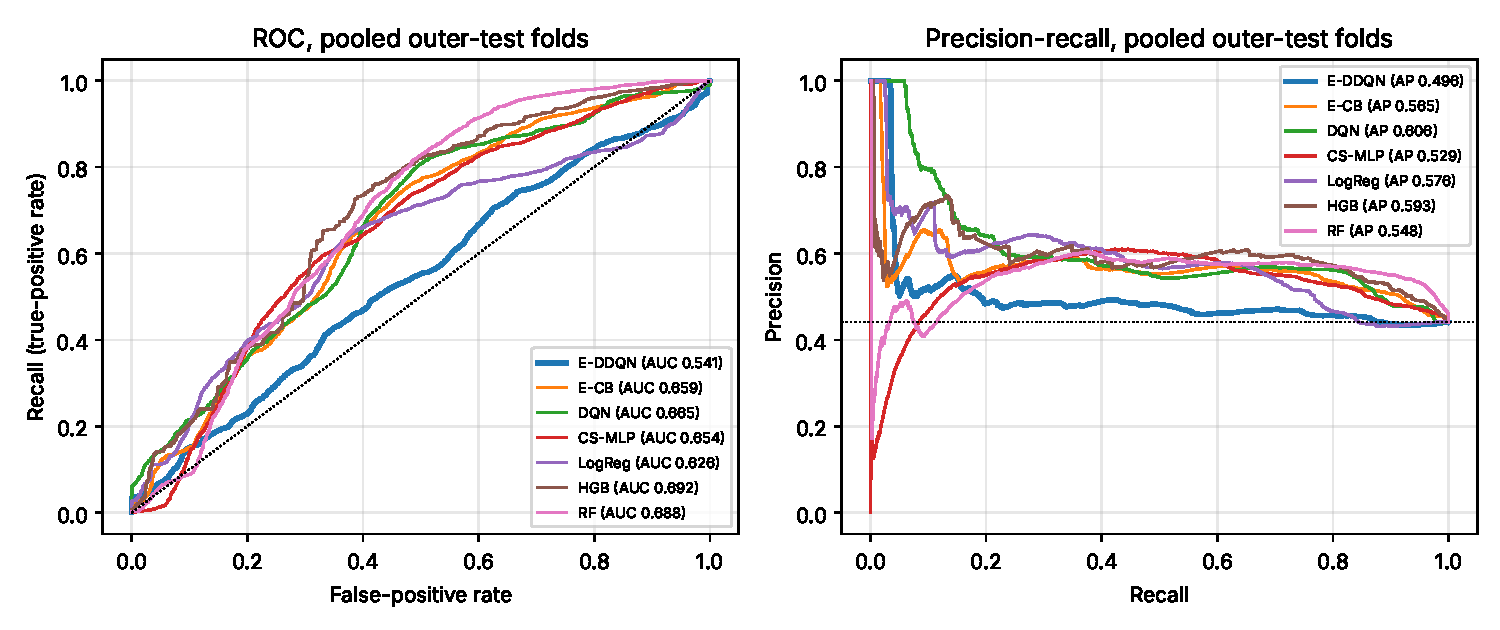
\includegraphics[width=\textwidth]{figs/roc_pr_main.pdf}
\end{center}
